\documentclass[acmsmall,nonacm]{acmart}
\makeatletter
\renewcommand\@formatdoi[1]{\ignorespaces}
\makeatother

\usepackage{subcaption}
\usepackage{float}
\usepackage{tabularx}
\usepackage{graphicx}
\usepackage{caption}


%%
%% \BibTeX command to typeset BibTeX logo in the docs
\AtBeginDocument{%
  \providecommand\BibTeX{{%
    \normalfont B\kern-0.5em{\scshape i\kern-0.25em b}\kern-0.8em\TeX}}}

% TODO is our font size no less than 10px?

\begin{document}

%\begin{titlepage}
%\end{titlepage}

%%
%% The "title" command has an optional parameter,
%% allowing the author to define a "short title" to be used in page headers.
\title{AI Dependability Assessment} % TODO find a good title

%%
%% The "author" command and its associated commands are used to define
%% the authors and their affiliations.
%% Of note is the shared affiliation of the first two authors, and the
%% "authornote" and "authornotemark" commands
%% used to denote shared contribution to the research.

\author{Patrick Deutschmann}
\email{patrick.deutschmann@student.tugraz.at}

\author{Lukas Timpl}
\email{lukas.timpl@student.tugraz.at}


%%
%% The abstract is a short summary of the work to be presented in the
%% article.
\begin{abstract}
% TODO write abstract
\end{abstract}

%%
%% The code below is generated by the tool at http://dl.acm.org/ccs.cfm.
%% Please copy and paste the code instead of the example below.
%%
%\begin{CCSXML}
%<ccs2012>
%   <concept>
%       <concept_id>10010147.10010178.10010179</concept_id>
%       <concept_desc>Computing methodologies~Natural language processing</concept_desc>
%       <concept_significance>500</concept_significance>
%       </concept>
% </ccs2012>
%\end{CCSXML}

%%
%% This command processes the author and affiliation and title
%% information and builds the first part of the formatted document.
\maketitle

\tableofcontents


\section{Introduction}

This is a submission to the \textit{Siemens AI Dependability Assessment}\footnote{\url{https://ecosystem.siemens.com/ai-da-sc}}. The challenge task was to solve a 2D binary classification problem, i.e. a binary function $f(\mathbf{x})$ classifies a data point $\mathbf{x_i} = (x_i^1, x_i^2)$ as either $l_i=0$ (green) or $l_i=1$ (red). With only two dimensions, the data sets are rather simple, yet the approach should also scale to inputs of higher dimensions. Most importantly, however, $f(\mathbf{x})$ should provide safety guarantees. This means that the ML model must not only have high predictive capabilities but also be capable of producing provably reliable results under certain assumptions. Furthermore, the setting is chosen such that misclassification costs are not equal for the two classes. Following the analogy of traffic lights, it is more dangerous (costly) to classify a red sample as green than classifying a green sample as red. It is given that the training data is labelled correctly and that the classes do not overlap.  

Our solution aims at striking the ideal balance of these criteria in that it displays high predictive performance, gives provable safety guarantees, scales well to more complex data sets, and lets domain experts dynamically configure the class-wise cost of misclassification.

The architecture we chose is a deep neural network trained with cost-weighted binary cross-entropy loss. The safety guarantees follow the assumption of reliable training inputs. Using Linear Relaxation Based Perturbation Analysis (LiRPA), we can guarantee stable predictions in the $\epsilon$-neighbourhood of previously seen samples.

\subsection{Data sets}

Fig. \ref{fig:datasets} shows the three data sets of the challenge. Before we started our experiments, we analysed them and found that they differ in multiple critical aspects. 

\begin{enumerate}
	\item \textbf{Size}: The data sets vary in size, with A being the smallest and C the biggest.
	\item \textbf{Class balance}: While data set B is relatively balanced, A and C show significant imbalance with a ratio of roughly 2:1 and 10:1, respectively, where class 0 (green) is the overrepresented one.
	\item \textbf{Separability}: It is easy to see that data set B can be separated by drawing a simple sine-like wave across the two dimensions and data set B by using multiple ellipses. For data set A, however, it is harder to make out a clear trend. There are several cases where green and red samples are very close to each other, and accurately separating classes will prove difficult.
\end{enumerate}

Thus, while we employ the same general approach for all three data sets, we tune our hyper-parameters separately to obtain ideal performance. We use simpler models for smaller data sets to prevent overfitting and counter class imbalance by using a weighted loss, as detailed in Section \ref{sec:approach}. % TODO really true that we use simpler model for data set A?

% TODO exchange colours for classes in plots

\begin{figure}
\centering
\begin{subfigure}{.32\textwidth}
  \centering
  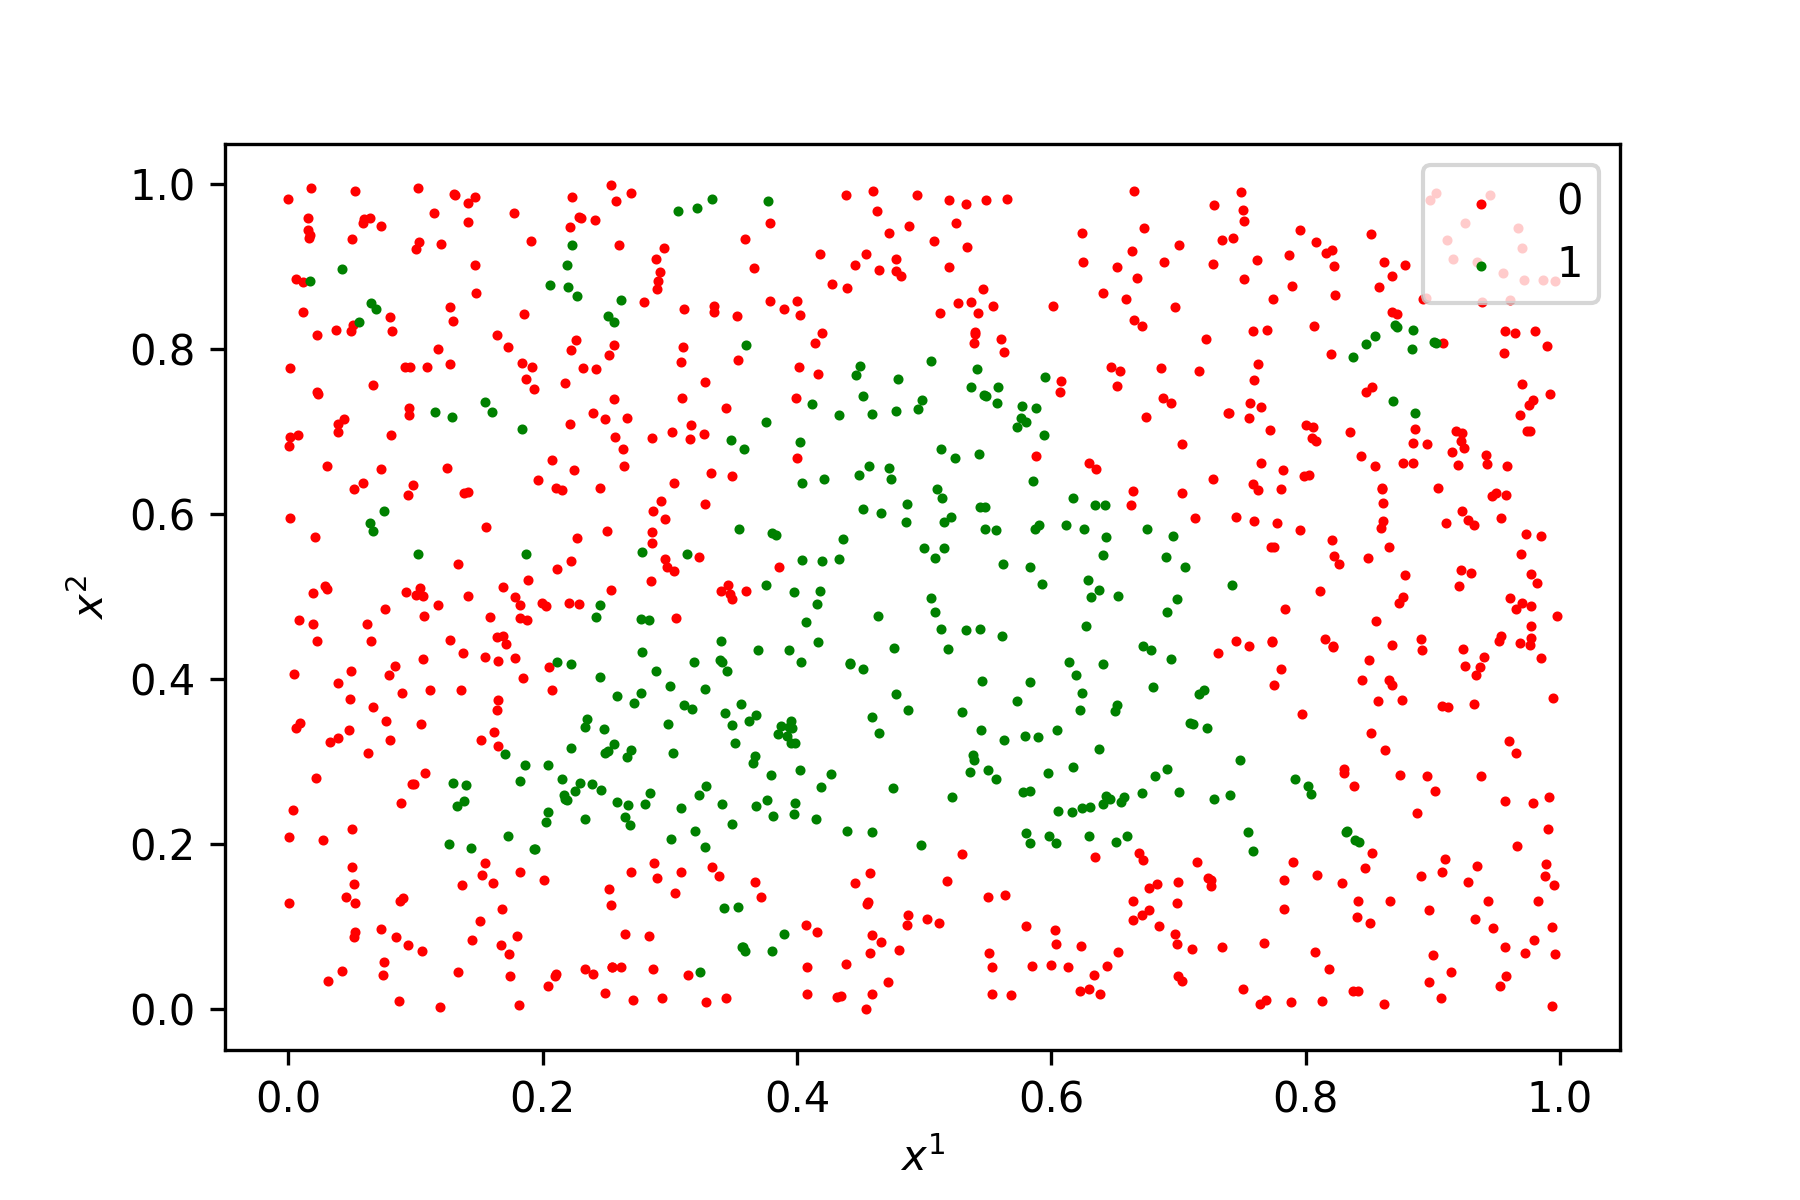
\includegraphics[width=\textwidth]{assets/ds_a.png}
  \caption{1,000 samples}
\end{subfigure}
\begin{subfigure}{.32\textwidth}
  \centering
  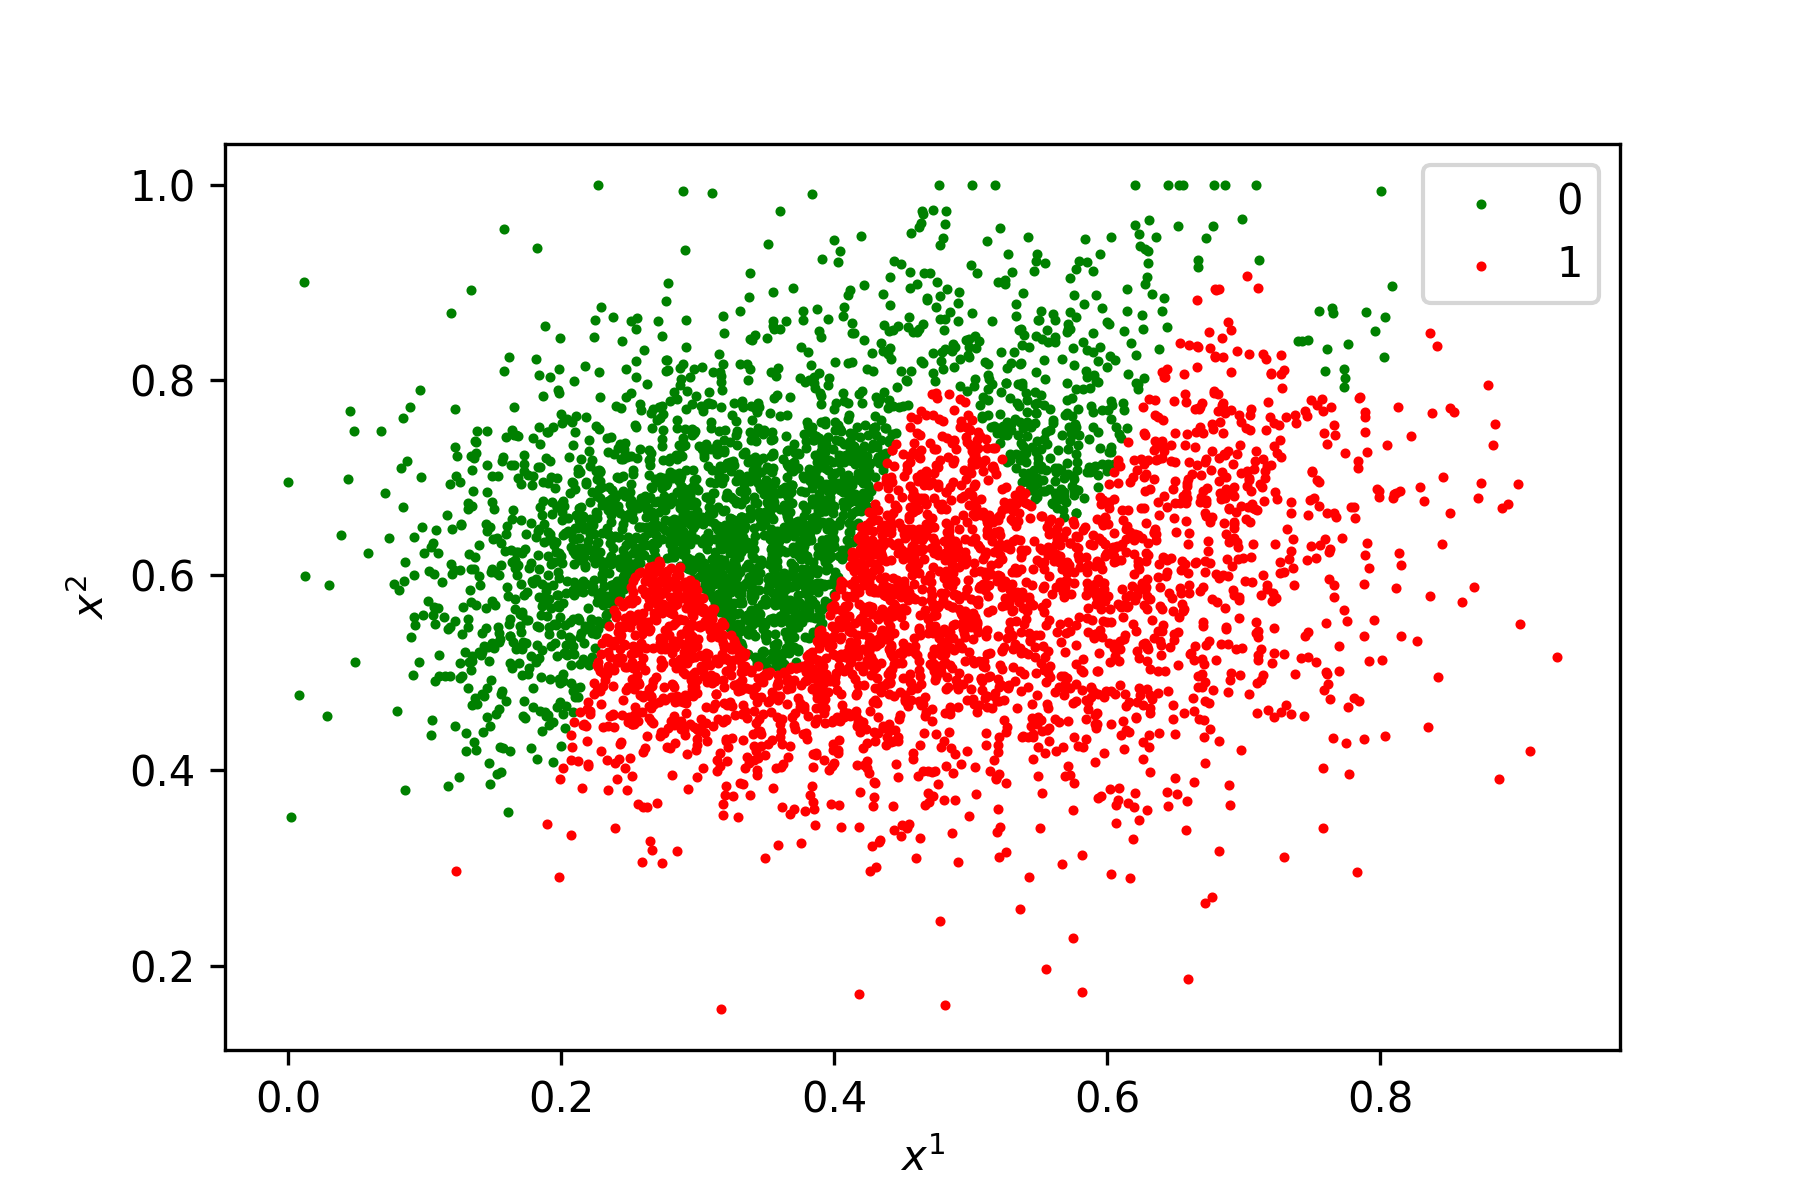
\includegraphics[width=\textwidth]{assets/ds_b.png}
  \caption{5,000 samples}
\end{subfigure}
\begin{subfigure}{.32\textwidth}
  \centering
  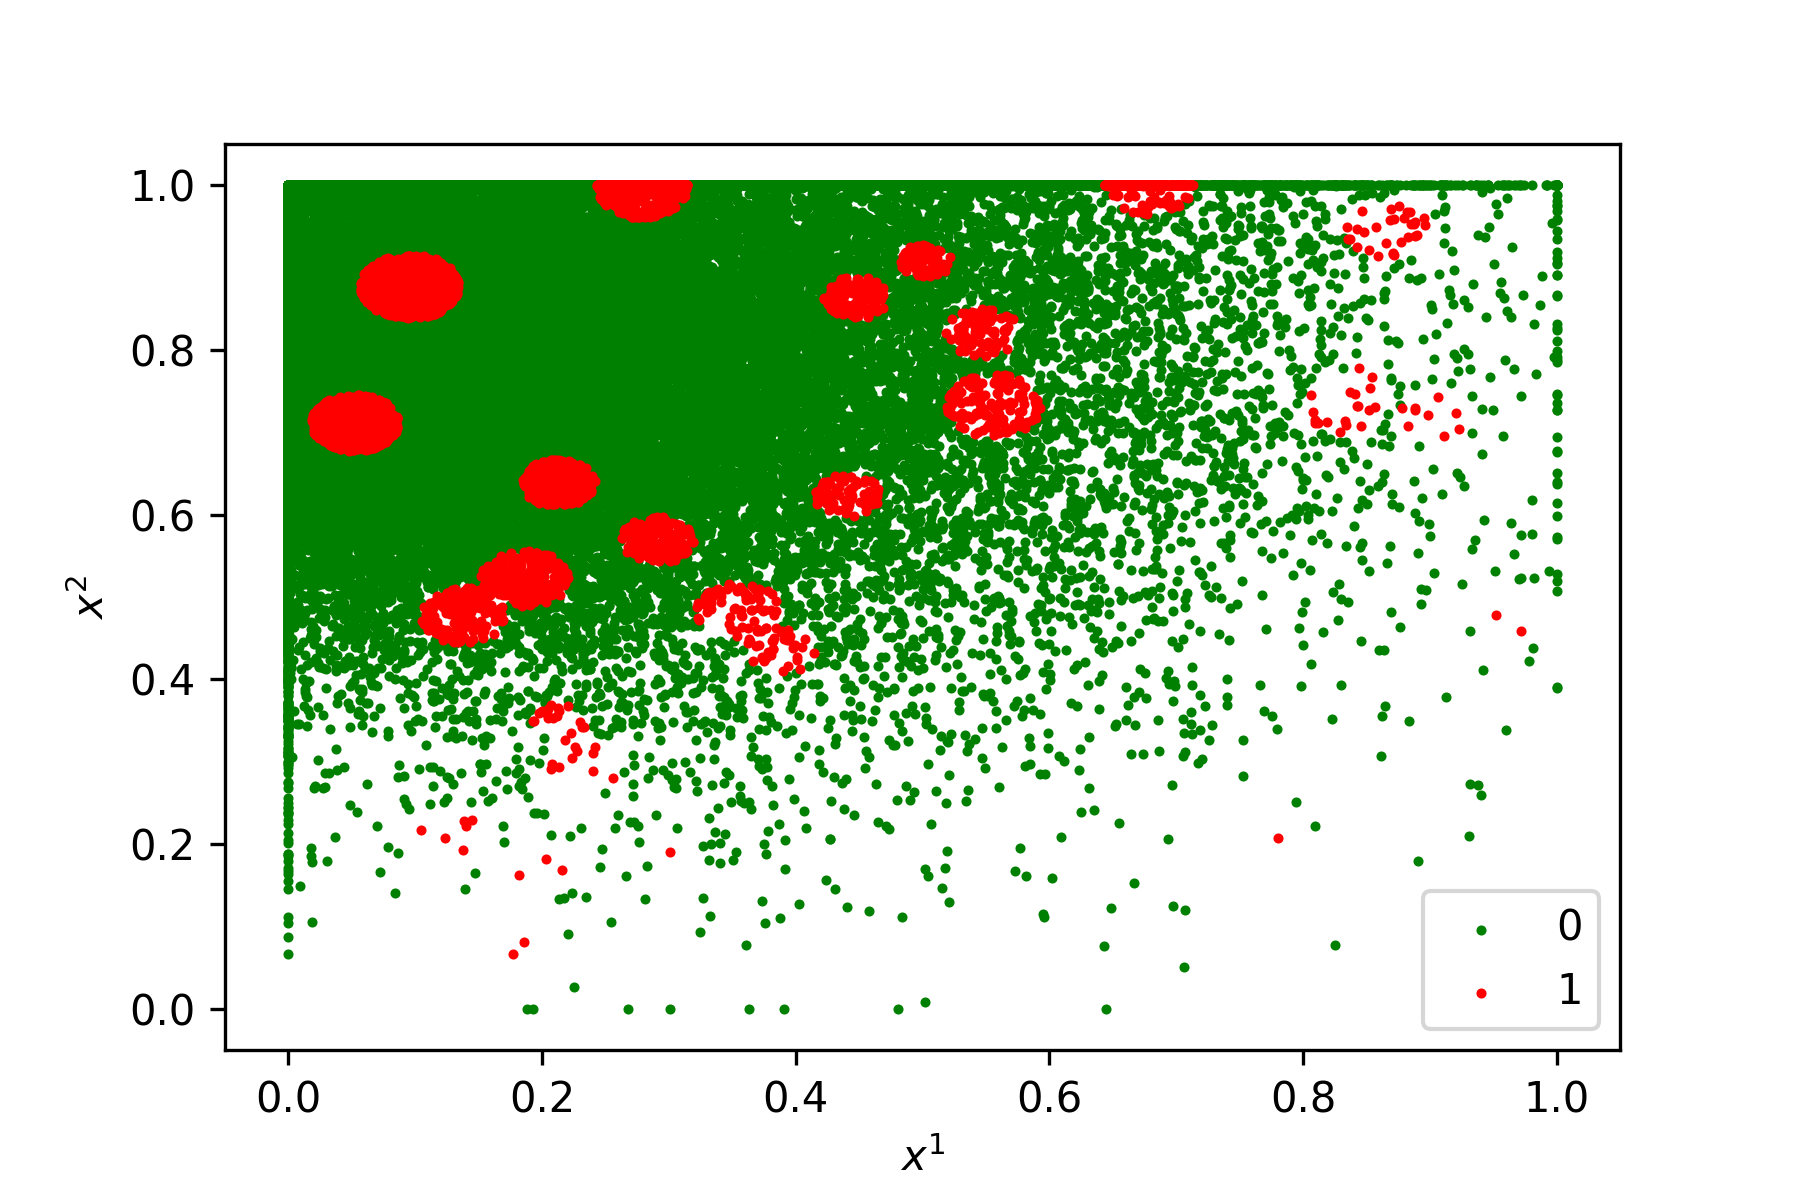
\includegraphics[width=\textwidth]{assets/ds_c.png}
  \caption{50,000 samples}
\end{subfigure}
\caption{The data sets of the challenge differ significantly in size, class balance and separability.}
\label{fig:datasets}
\end{figure}


\section{Possible Solutions and Related Work}

Before choosing an approach, we analysed the core aspect of safety guarantees and possible assumptions. In particular, we looked at two possibilities of formulating guarantees for our problem: (a) expressing uncertainty for a given sample and (b) robustness against local perturbations. 

The former addresses the problem that most machine learning approaches always produce an answer, even if they encounter inputs the like of which they have never seen before. In that case, they should be highly unsure about their prediction but mostly fail to express that. One way to counter this are Bayesian Neural Networks (BNNs) \cite{goan2020bnn}. In a probabilistic approach, they place a distribution over the network parameters. They can, hence, express their uncertainty in case they see challenging inputs. This could be very useful in a security-critical environment and would, for instance, allow an autonomous vehicle to alert its driver if it is unable to deal with a particular situation. However, it does not strictly correspond to the challenge description where security guarantees for unseen inputs should be made. A BNN would require a concrete input $\mathbf{x}_i$ to express its certainty.

Therefore, we to decided pursue the goal of (b), meaning that we made our model robust against local perturbations. Simply put, this means that the model should reliably label unseen samples that lie near known training samples with the same class as the known sample. We put forward a more formal definition in Section \ref{sec:approach}. It is trivial to give such guarantees for simple models: For logistic regression and k-nearest-neighbours, the decision boundary can be used to derive them. For naive Bayes classifiers, confidence intervals can be directly computed. Some of these classifiers would also produce relatively well on the given datasets, which is why we use them as baselines for our final model (see Subsection \ref{ssec:baselines}). However, they would not scale well to higher dimensions and more complex problems. 

More complicated models include SVM and Gaussian Processes (GP) for classification. SVM can be powerful, especially with RBF kernels, but cannot provide the guarantees we require. GP would provide us with empirical confidence intervals but becomes inefficient in higher dimensions. Furthermore, both approaches are not leading in state-of-the-art predictive capabilities for challenging tasks, especially in the vision domain.

Another powerful class of machine learning models are decision trees and random forests. They display high predictive capabilities and can also be verified, but as \cite{tornblom2018formal} found, verification time does not scale very well to larger models.

Finally, we arrive at deep neural networks, which have received much attention in recent machine learning history. They scale well to very complex problems but used to be considered textbook examples for black-box models. However, recently, there has been a lot of work focused on explainability and defence against adversarial samples. It started with approaches that provided exact upper and lower bounds for neural network outputs given certain input perturbations. Reluplex \cite{katz2017reluplex} is an example that, however, only works for networks with ReLU activations. Further research introduced methods that work with arbitrary activations and use linear relaxations that compute tight approximations to significantly improve performance, allowing these techniques to be scaled to larger networks. Such work includes IBP \cite{gowal2019effectivenessIBP}, CROWN \cite{zhang2018efficient} and DeepPoly \cite{singh2019abstractDeepPoly}. We decided to use AutoLiRPA \cite{xu2020autoLiRPA} that introduces a framework that applies these techniques to general neural networks and allows for automatic analysis on computational graphs.

\subsection{Baselines} \label{ssec:baselines}

% TODO add our baselines



\section{Approach} \label{sec:approach}
%TODO
%• A description of the employed ML approach
%• All assumptions made, including an exhaustive proposal/justification for their validation
~\cite{xu2020automatic}


Relying on the assumption that our training samples are correctly labelled, we want to guarantee for a certain number of samples, which we call \textit{verified}, that all inputs surrounding them are assigned the same class as the centre. Formally, we define a neighbourhood around training sample $\mathbf{x}_i$ as an $L_p$-ball with radius $\epsilon$. We then guarantee for all possible (infinitely many) samples that lie within this ball $\{\mathbf{y} \in \mathbb{R}: ||\mathbf{x}_i - \mathbf{y}||_p < \epsilon \}$ that they are assigned $l_i$. In our implementation, we support $L_2$ and $L_\infty$-norm.

\section{Experiments}
%TODO
% For each data set, an upper bound for the misclassification error, including its justification

\subsection{Metrics}

\subsection{Results}
We used Weights \& Biases \cite{wandb} for experiment tracking and visualisations.


\section{Scaling to higher dimensions}
%TODO
% An outline how the approach could be scaled to higher dimensions

\section{Appendix}
%TODO
% In an appendix, the documented code should be supplied

\pagebreak  

%%
%% The next two lines define the bibliography style to be used, and
%% the bibliography file.
\bibliographystyle{ACM-Reference-Format}

\bibliography{references}
% References to results that are used


\end{document}
\endinput

